\documentclass[12pt]{article}

%
% FILL OUT THIS SECTION
% 
\author{Arthea Valderrama}
\date{August 2023}



% Packages
\usepackage[T1]{fontenc} % Some font fixes
\usepackage{amsmath, amssymb, amsthm} % Allows extra math commands
\usepackage{listings} % Allows importing code
\usepackage{subcaption} % Helps with figures
\usepackage{graphicx} % Allows including images
\usepackage{float}
\usepackage[dvipsnames,table]{xcolor} % Helps with manipulating colors
\usepackage{hyperref} % Link to web pages
\usepackage[legalpaper, margin=1in]{geometry} % Adjusts page margins
\usepackage{subcaption}


% Settings for portfolio
\title{Embedding Python Models in Xspec}


% Formatting style for code
\definecolor{backcolour}{rgb}{0.92,0.92,0.90}
\lstdefinestyle{cppcode}{
	language=c++,
	%basicstyle=\footnotesize\ttfamily,
	basicstyle=\ttfamily,
	commentstyle=\color{Green},
	tabsize=4,
	columns=flexible,
	keepspaces=true,
	numbers=left,
	keywordstyle=\color{Blue},
	stringstyle=\color{Maroon},
	showstringspaces=false,
	backgroundcolor=\color{backcolour},
	frame=single,
	breaklines=true
}
\lstset{style=cppcode}
% Get images from figures directory
\graphicspath{ {./figures/} }

\begin{document}

\maketitle

	Although recent AtomDB models are written in Python to ease development, spectral analysis is still largely done using C++ based XSPEC. Utilizing a C++ based code that can import Python models in XSPEC enables an astronomer access to newer models, without having to entirely write them in a different language. This document works with PyApec, as XSPEC already has a built-in Apec model, to utilize an embedded Python model. This is different from PyXSPEC, which uses XSPEC from a Python terminal, while embedding a Python model entails C++ code to call a built-in Python interpreter to run Python code.

\section{Installation} 

For now, this method works using the default Python interpreter in a Linux system, not on something similar to the Anaconda version of Python. It is important to have the XSPEC software, as well as the HEASOFT package, which are available at \url{https://heasarc.gsfc.nasa.gov/docs/software/lheasoft/}. The following procedure should work as long as HEASOFT is installed and ready, meaning that it is initliazed in the environment and typing 'xspec' at the command terminal will start the software.  

\subsection{Modifying Python Code} \label{python}
Some edits to Python code must be made first. Any calls to \texttt{import xspec} must be removed due to circular dependency. Additionally, Python code that creates parameters for Python models should also be removed. 

\subsection{Modifying the Makefile}\label{Makefile}
Firstly, wherever HEASOFT is installed, change into that directory. Then, change into the directory that XSPEC uses to create Makefiles for custom models. \newline
\indent\texttt{ > cd Xspec/src/tools/initpackage} \newline
It is recommended you know the location of your Python include directory and your Python library path. To find the Python include directory, run and open a Python terminal on your system as follows:\newline
\indent \texttt{>import sys} \newline
\indent\texttt{>from distutils.sysconfig import get\_python\_inc}\newline
\indent\texttt{>python\_include\_dir = get\_python\_inc()}\newline
\indent\texttt{>print("Python Include Directory:", python\_include\_dir)}\newline
The result printed is the Python include directory, which may look something like \newline
\texttt{-I/usr/include/python3.9}. The -I flag before the Python include directory is imperative to linking the Makefile. To find the Python library path on your system, run and open a python terminal as follows:\newline
\indent\texttt{>import sysconfig}\newline
\indent\texttt{>python\_paths = sysconfig.get\_paths()} \newline
\indent\texttt{>python\_lib\_dir = python\_paths['platstdlib']}\newline
\indent\texttt{>print("Python Library Directory:", python\_lib\_dir)}\newline
The result may look something like \texttt{-L/usr/lib64/python3.9}. The -L flag before that path is important in linked to the Makefile. It will also need a link to the version of Python being ran, i.e, "\texttt{-lpython3.9}", but it may vary depending on Python versions, so if it was Python3.6 it would then change to "\texttt{-lpython3.6m}" or so. \newline

Using a text editor, open the \texttt {xspackage.tmpl} document. Under the \texttt{HD\_CXXFLAGS} section, type in your Python include director preceded by "-I", followed by a space and a "\textbackslash." Under the \texttt{HD\_SHLIB\_LIBS} section, type in your Python version preceded by "-l", and your Python library path preceded by a "-L" then followed by a space and a "\textbackslash" to signify the end of line. 
\begin{figure}[H]
	\centering
	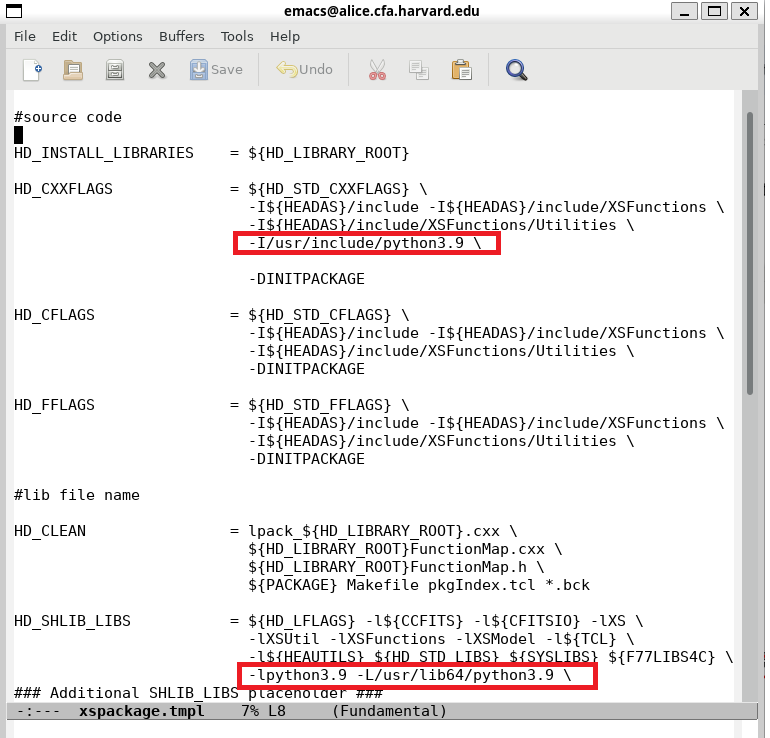
\includegraphics[width = 15cm] {makefile}
	\caption{sample Makefile that links to proper Python libraries and directives, highlighted in red}
\end{figure}

Save the changes, and change up one directory ("\texttt{cd ..}", making sure you are in \texttt{Xspec/src/tools}), then run "\texttt{hmake}" and "\texttt{hmake install}". This changes the Makefile so that now all local models will have these changes and the proper linkage to the Python interpreter in  XSPEC. 
\subsection{Making a local model}\label{model}
If modifying the Makefile worked out correctly, you should now be able to run and write Python code for XSPEC. More information on making a custom model can be found at \url{https://heasarc.gsfc.nasa.gov/xanadu/xspec/manual/XSappendixLocal.html}. \newline
In summary, one must have a \texttt{.dat} file detailing the model and its parameters (the file should contain the name of the model and the name of the model function) and at least one \texttt{.cpp} file with the main function being an extern "C" void function with the same name as the function outlined in the \texttt{.dat} file. Attached below is a sample C++ wrapper. \newline
\lstinputlisting{Codebase/wrapper.cpp}
The first line indicates the Python include directive, which may vary by your version of Python. A C++ class is used to contain the Python interpreter object, which is then called by the model routine function. The constructor initializes the C++ Python interpreter, imports numpy, and attempts locates the name of your python script module depending on the directory in which the file is located. The bulk of the conversion of data is located in the \texttt{caller()} function, which converts data values from C++ to Python, performs a function call to an embedded Python interface, and returns the data values from python back to C++ in a \texttt{RealArray\& Flux}. It then cleans up all of the objects created, and the destructor frees up the class object once ran. \newline
For the purposes of this tutorial, the directory of the location in which the custom model is held also contains a \texttt{.py} file for the python script to be imported. Creating a model for example would be as follows: \newline
\indent\texttt{>initpackage <modelname> model.dat .}\newline
\indent\texttt{>hmake}\newline
When you type in \texttt{ls} into the terminal, a list of files created by initpackage should be shown. The most important one to note is the \texttt{lpack\_<modelname>.cxx}. Open that file with a text editor, and add \texttt{\#include <dlfcn.h>} to the libraries. Inside the first function, add the following line:\newline
\indent\texttt{dlopen("lib<yourversionofpython>.so", RTLD\_LAZY | RTLD\_GLOBAL);}
\begin{figure}[H]
	\centering
	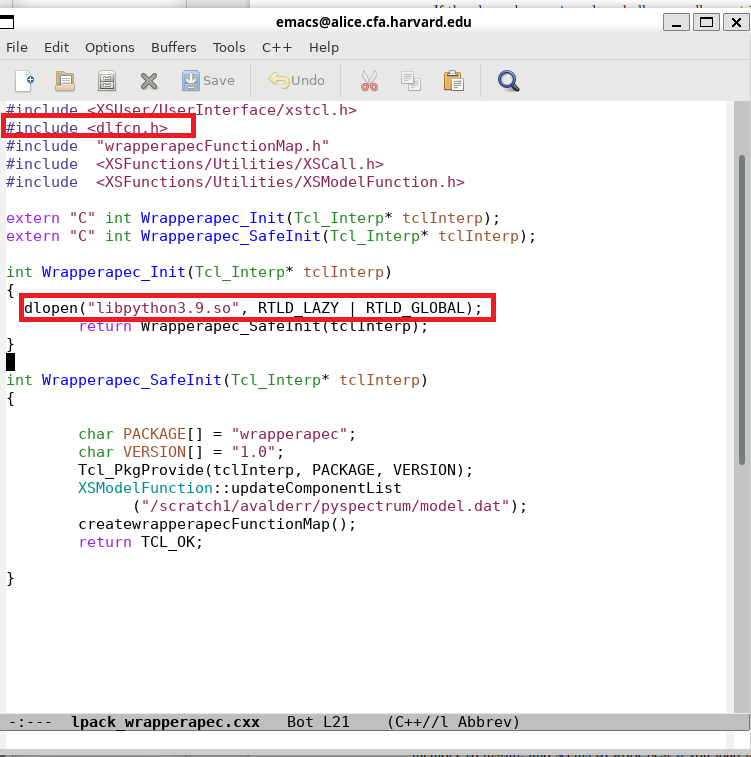
\includegraphics[width = 15cm] {lpack}
	\caption{Sample lpack\_<modelname>.cxx file edited, highlighted in red. }
\end{figure}
 It should be noted that if you have an earlier version of Python, i.e Python3.7 to also include the "m" that supercedes that version. Some earlier versions of Python would be written as "libpython3.6m.so" to work. This is important in importing Python modules like numpy into XSPEC. \newline
Ideally all the changes should allow one to import and run their custom embedded Python model into XSPEC. Open XSPEC, and load the model as follows: \newline
\indent\texttt{xspec>lmod <modelname> /path/to/local/model}\newline
The model should load successfully! Now you can use it and treat it as any other XSPEC model. 

\section{Usage}
Ideally, embedded Python models properly load into XSPEC without unexpected core dumps or improper linkage issues. Inside XSPEC, and typing in the "\texttt{model}" command allows you to view the list of models that XSPEC has loaded in that section. Your custom routine function name should be listed, followed by an \texttt{*} indicating that it is an imported model. Running the model command again followed by the name of your custom routine will initialize the model to be used in spectral analysis, as you will later be provided with the prompt to input parameters as listed in the custom \texttt{.dat} file. \newline

In the context of speed, fitting times vary between routines such as the built-in model in XSPEC, Python models, and embedded Python models. 
\begin{figure}[H]
\centering
\begin{subfigure}{0.49\textwidth}
\centering
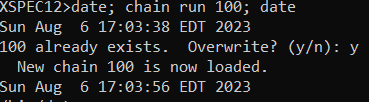
\includegraphics[width = \textwidth]{apecbenchmark}
\caption{Benchmark of an apec model running 100 different fits }
\label{fig:left}
\end{subfigure}
\begin{subfigure}{0.49\textwidth}
\centering
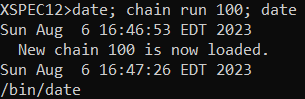
\includegraphics[width = \textwidth]{pyapecbenchmark}
\caption{Benchmark of an embedded model running 100 different fits}
\label{fig:right}
\end{subfigure}
\label{fig:combined}
\end{figure}

\begin{figure}[H]
	\centering
	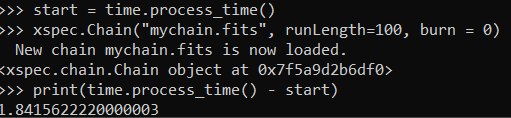
\includegraphics[width = 10cm]{python}
	\caption {Benchmark of apec model in Python running 100 different fits}
	\label{fig:left}
\end {figure}

The embedded Python model in XSPEC is slower than the C++ built-in model, but by an approximate factor of 2 due to the data conversions between C++ and Python. Purely running Python is the fastest route. While these benchmarks show differences in speed between the routines, there should not be a significant noticeable difference running models one at a time. 

\section{Acknowledgements}
In the process of discovering this method to load Python models into regular XSPEC, I have run into many unexpected core dumps and memory issues. Potentially the largest issues I have come across is importing numpy into XSPEC, and trying the method with Anaconda Python. I would like to thank Adam Foster and Nancy Brickhouse for advising me throughout this process and guiding me through XSPEC. I would also like to thank Craig Gordon for assisting me with debugging and rewriting XSPEC to run a Python interpreter. Lastly, internet sources such as StackOverflow and the official Python/C documentation (which can be found here:\url{https://docs.python.org/3/extending/embedding.html}) were essential in helping me figure out this process. 
 \newline

\newpage

% ADD INCLUDES FOR PROJECTS HERE




\end{document}
